\documentclass[10pt,landscape,a4paper]{article}
\usepackage[utf8]{inputenc}
\usepackage[nosf]{kpfonts}
\usepackage[t1]{sourcesanspro}
% \usepackage[lf]{MyriadPro}
% \usepackage[lf,minionint]{MinionPro}

% For the multiple columns in the cheat sheet
\usepackage{multicol}

% Set the margins of the paper
\usepackage[top=0mm,bottom=1mm,left=0mm,right=1mm]{geometry}

% To use colours
\usepackage{xcolor}

% To typeset small fonts
\usepackage{microtype}

% To include graphics
\usepackage{graphicx}

\graphicspath{ {./images/} }

\let\bar\overline

\definecolor{myblue}{cmyk}{1,.72,0,.38}

\everymath\expandafter{\the\everymath \color{myblue}}
\everydisplay\expandafter{\the\everydisplay \color{myblue}}

\renewcommand{\baselinestretch}{.8}
\pagestyle{empty}

\makeatletter
\renewcommand{\section}{\@startsection{section}{1}{0mm}%
  {.2ex}%
  {.2ex}%x
  {\color{myblue}\sffamily\small\bfseries}}
\renewcommand{\subsection}{\@startsection{subsection}{1}{0mm}%
  {.2ex}%
  {.2ex}%x
  {\sffamily\bfseries}}


\makeatother
\setlength{\parindent}{0pt}

\begin{document}
\small
\begin{multicols*}{5}
  \raggedcolumns


  \section{Kinematics}

  Equations of motion: \\
  \(s = ut + \frac{1}{2} at^2\) \\
  \(v = u + at\) \\
  \(v^2 = u^2 + 2as\)

  Relative velocity: \\
  \(\vec{v}_{PA} = \vec{v}_{PB} + \vec{v}_{BA}\)

  Maximum height (no air resistance): \\
  \(h_{max} = \frac{u^2 \sin^2 \theta}{2g}\), where \(\theta\) is the angle to the ground.

  Range (no elevation change \& no drag): \\
  \(R = \frac{u^2 \sin 2 \theta}{g}\), where \(\theta\) is the angle to the ground.

  \subsection{Vector resolution}
  \(\cos \theta\) stands for closing the angle \(\theta\), so the vector that closes the angle is \(\cos \theta\) and the vector that opens the angle is \(\sin \theta\).


  \section{Newton's laws}

  Newton's second law: \\
  \(F_{net} = ma\) \\
  \(F_{net} = \frac{d \vec{p}}{dt} = \frac{d (m \vec{v})}{dt}\)

  Newton's second law for variable mass: \\
  \(F_{net} = ma + \vec{v}_{rel} \frac{dm}{dt}\)

  Laminar flow drag: \\
  \(F_D = bv\)

  Turbulent flow drag: \\
  \(F_D = kv^2\)

  Terminal velocity: \\
  \(v(t) = \frac{mg}{b} \left(1 - e^{-\frac{bt}{m}} \right)\)


  \section{Circular motion}

  Arc length: \\
  \(s = r \theta\), where \(\theta\) is in radians.

  Angular displacement: \\
  \(\theta = \frac{s}{r}\)

  Frequency: \\
  \(\frac{1}{T}\), where \(T\) is the period.

  Angular velocity: \\
  \(\omega = \frac{d \theta}{dt} = 2 \pi f = \frac{2 \pi}{T} = \frac{v_{tan}}{r}\)

  Angular acceleration: \\
  \(\alpha = \frac{d \omega}{dt}\)

  Centripetal acceleration: \\
  \(a = \frac{v^2}{r} = r \omega^2 \)

  Total linear acceleration: \\
  \(\vec{a} = \vec{a}_{tan} - \frac{(\vec{v}_{tan})}{R}^2 \hat{r} = \vec{a}_{tan} - R \omega^2 \hat{r}\)

  Angular quantities: \\
  \(s = r \theta\) \\
  \(v_{tan} = r \omega\) \\
  \(a_{tan} = r \alpha\)

  Equations of motion: \\
  \(\omega_f = \omega_i + \alpha t\) \\
  \(\theta - \theta_0 = \omega_i t + \frac{1}{2} \alpha t^2\) \\
  \(\omega_f^2 = \omega_i^2 + 2 \alpha (\theta - \theta_0)\)

  Non-uniform circular motion: \\
  \(\vec{a} = \vec{a}_r + \vec{a}_{tan}\)


  \section{Work, Energy, Power}

  Work done: \\
  \(W = \vec{F} \cdot \vec{s} = Fs \cos \theta\) \\
  \(W = \int_a^b \vec{F} \cdot d \vec{l}\)

  Kinetic energy: \\
  \(KE = \frac{1}{2}mv^2\)

  Potential energy: \\
  \(\Delta U = - \int \vec{F} \cdot d \vec{l}\)

  Work-energy theorem: \\
  \(W = KE_f - KE_i\) \\
  \(W = \frac{1}{2}mv_f^2 - \frac{1}{2}mv_i^2\)

  Gravity: \\
  \(PE_{grav} = mgh = - \int \vec{F}_{grav} \cdot d \vec{l}\) \\
  \(PE_{grav} = - \frac{GMm}{r}\) \\
  \(F_{grav} = \frac{GMm}{r^2}\)

  Force: \\
  \(F = -\frac{dU}{dx}\)

  Springs: \\
  \(\vec{F}_{spring} = -k \vec{x}\) \\
  \(PE_{spring} = \frac{1}{2} kx^2\)

  Power: \\
  \(P_{avg} = \frac{\Delta W}{\Delta t}\) \\
  \(P = \frac{dW}{dt}\) \\
  \(P = \vec{F} \cdot \vec{v} = F v \cos \theta\)


  \section{Momentum}

  Momentum: \\
  \(\vec{p} = m \vec{v}, \quad p = mv\)

  Impulse: \\
  \(\vec{J} = \vec{F}_{net} \Delta t, \quad J = F_{net} \Delta t\) \\
  \(\vec{J} = \int_{t_1}^{t_2} \vec{F}_{net} \, dt\)

  Elastic collisions: \\
  \(v_A - v_B = v'_B - v'_A\)

  Coefficient of restitution \(e\): \\
  \(v'_B - v'_A = -e (v_B - v_A)\)

  Centre of mass (CM): \\
  \(x_{CM} = \frac{m_1x_1 + \ldots + m_nx_n}{m_1 + \ldots + m_n} = \frac{1}{M} \sum_{i = 1}^n m_i x_i\) \\
  \(x_{CM} = \frac{1}{M} \int x \, dm\)


  \section{Rotation of rigid bodies}

  Torque: \\
  \(\vec{\tau} = \vec{r} \times \vec{F}\) \\
  \(\tau = rF \sin \theta\)

  Net torque: \\
  \(\vec{\tau}_{net} = I \vec{\alpha}, \quad \tau_{net} = I \alpha\)

  Moment of inertia (MOI): \\
  \(I = m_1r_1^2 + m_2r_2^2 + \cdots = \sum_i m_i r_i^2\) \\
  \(I = \int r^2 \, dm\)

  Parallel axis theorem: \\
  \(I_P = I_{CM} + Md^2\)

  Perpendicular axis theorem (only for flat objects): \\
  \(I_z = I_x + I_y\)

  Rotational kinetic energy: \\
  \(KE_{rot} = \frac{1}{2} I \omega^2\)

  Work-energy theorem: \\
  \(W = \int \tau \, d \theta\) \\
  \(W = \frac{1}{2} I \omega_f^2 - \frac{1}{2} I \omega_i^2\)

  Power: \\
  \(P = \tau \omega\)

  Rolling without slipping: \\
  \(v_{CM} = R \omega\) \\
  \(KE_{total} = \frac{1}{2}mv_{CM}^2 + \frac{1}{2}I_{CM} \omega^2\)

  % Rectangular plate
  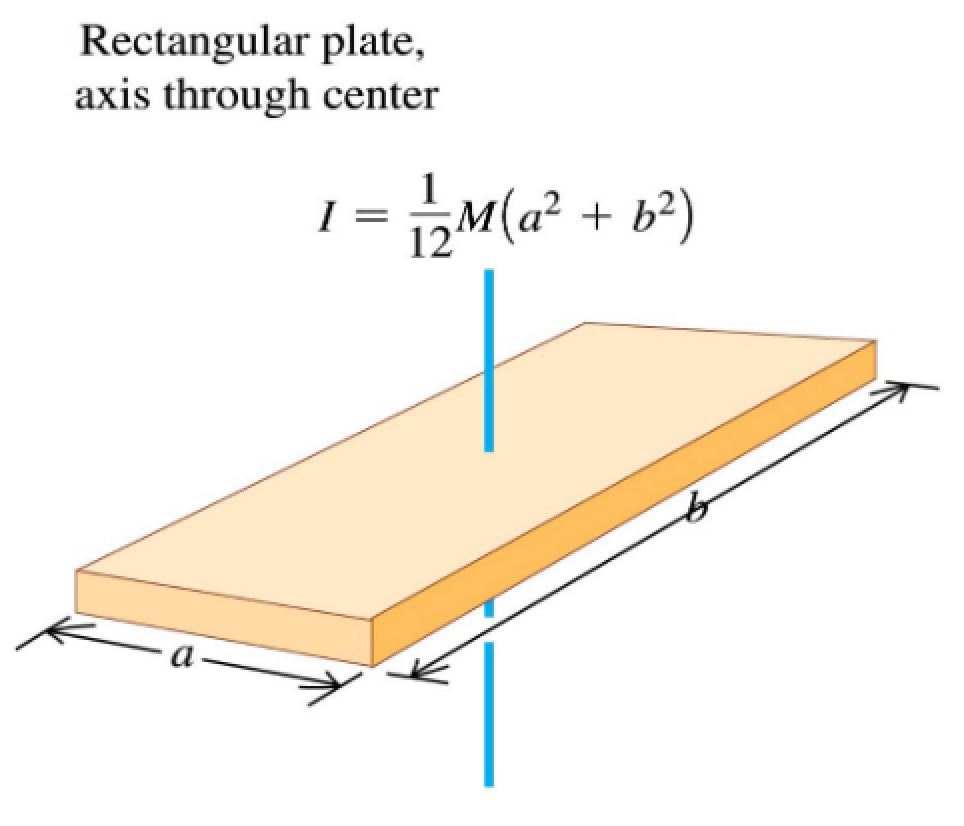
\includegraphics[width = 0.74\linewidth]{rectangular-plate-moi-1}
  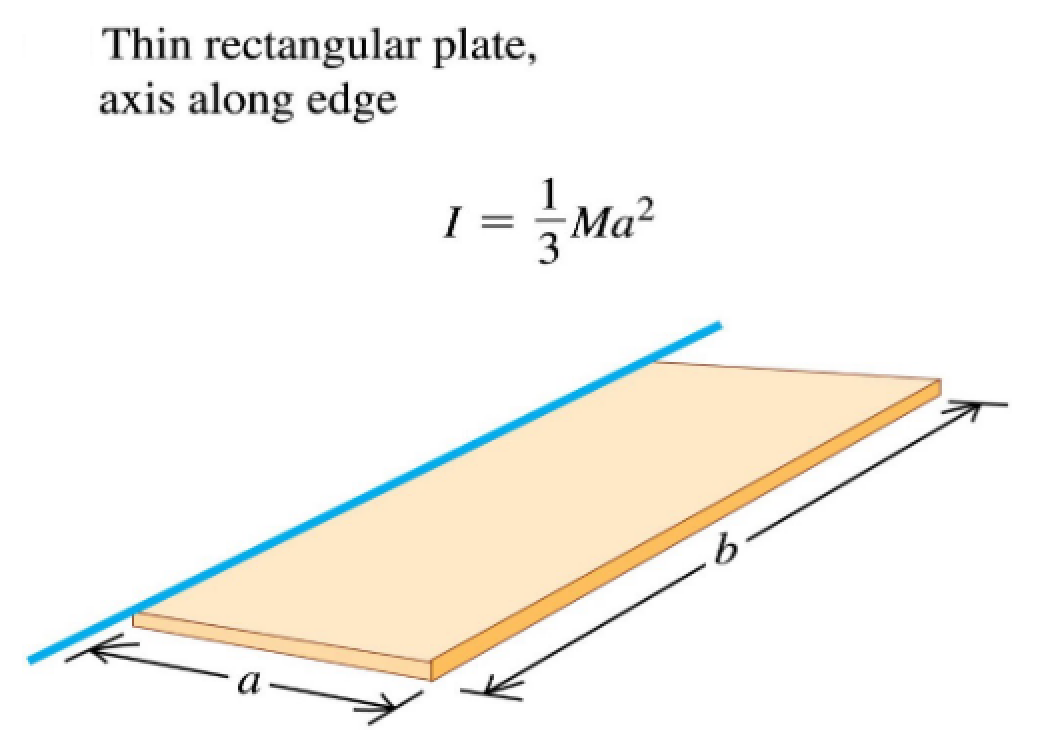
\includegraphics[width = 0.74\linewidth]{rectangular-plate-moi-2}

  % Sphere
  \begin{tabular}{c}
    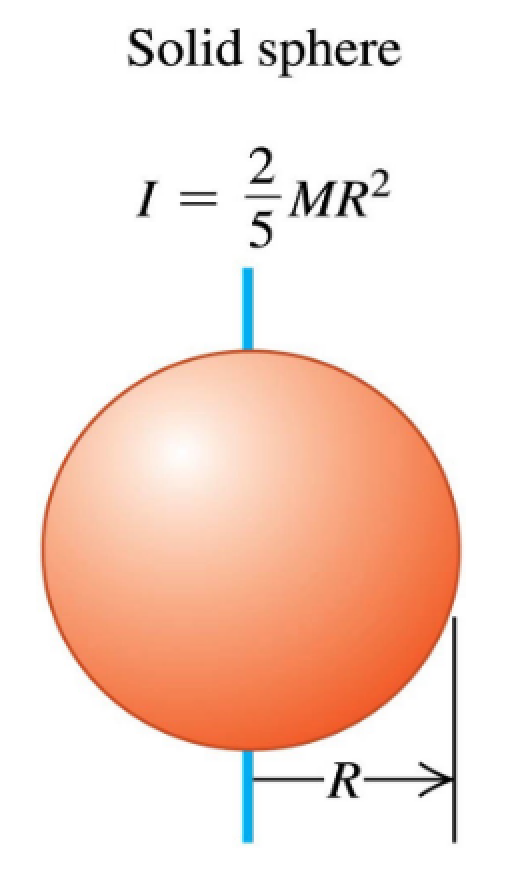
\includegraphics[width = 0.5\linewidth]{solid-sphere-moi}
    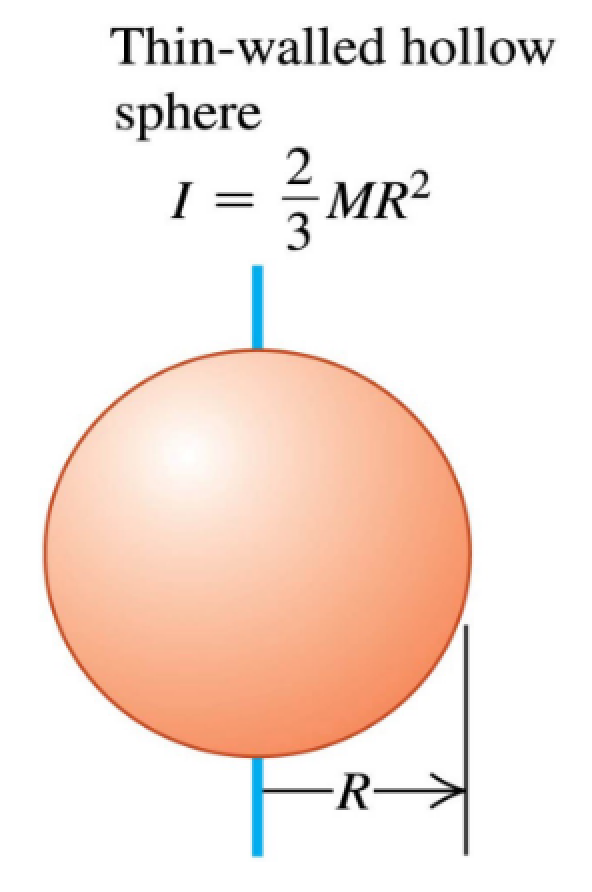
\includegraphics[width = 0.5\linewidth]{thin-walled-hollow-sphere-moi}
  \end{tabular}

  % Cylinder
  \begin{tabular}{c}
    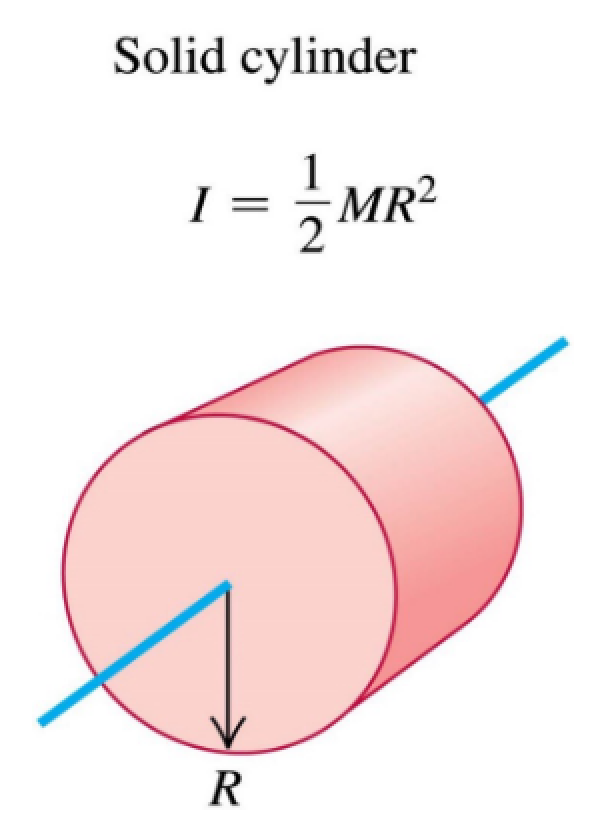
\includegraphics[width = 0.33333333333333\linewidth]{solid-cylinder-moi}
    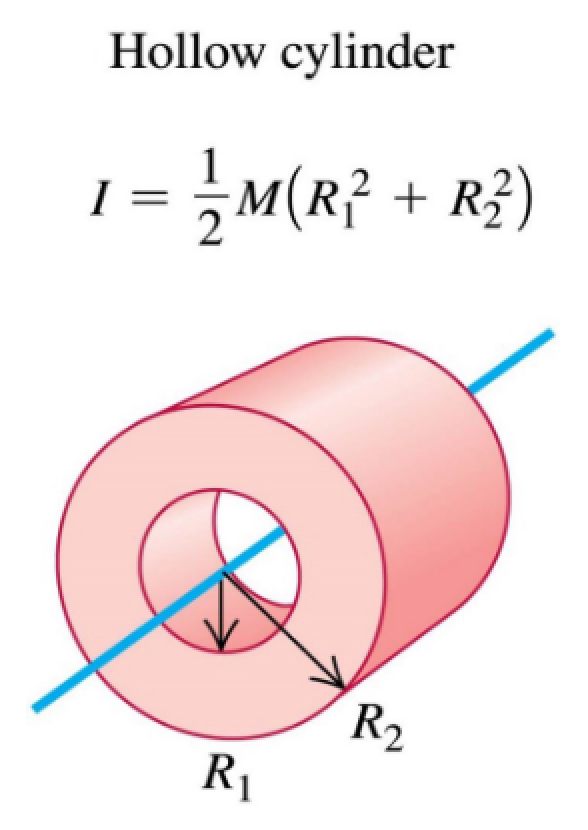
\includegraphics[width = 0.33333333333333\linewidth]{hollow-cylinder-moi}
    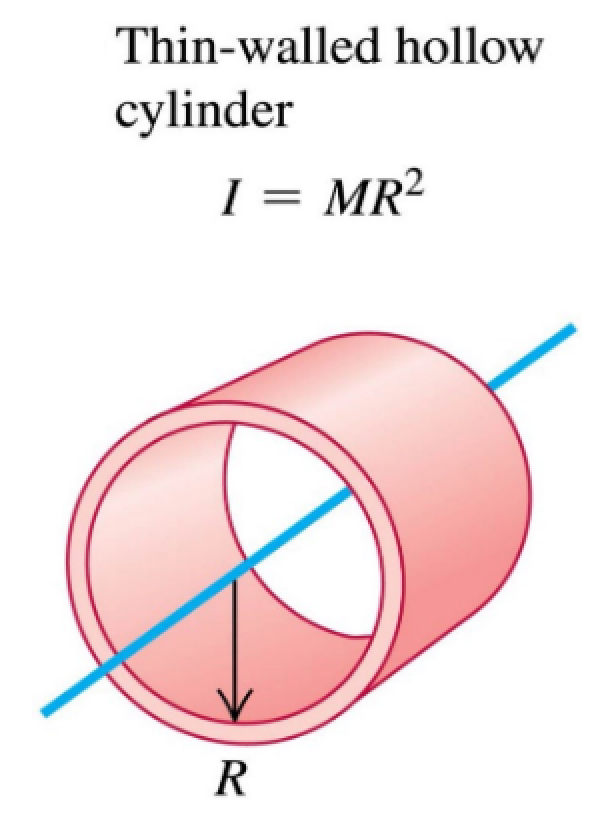
\includegraphics[width = 0.33333333333333\linewidth]{thin-walled-hollow-cylinder-moi}
  \end{tabular}

  % Slender rod
  \begin{tabular}{c}
    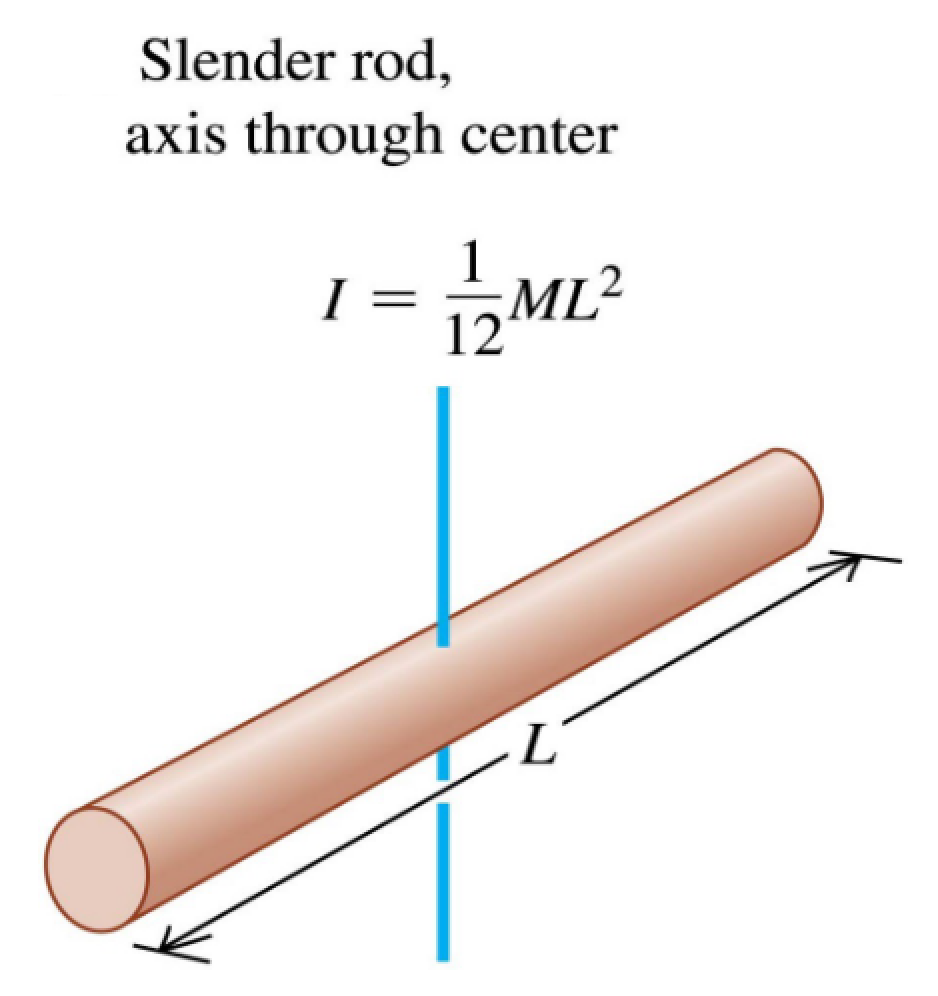
\includegraphics[width = 0.5\linewidth]{slender-rod-moi-1}
    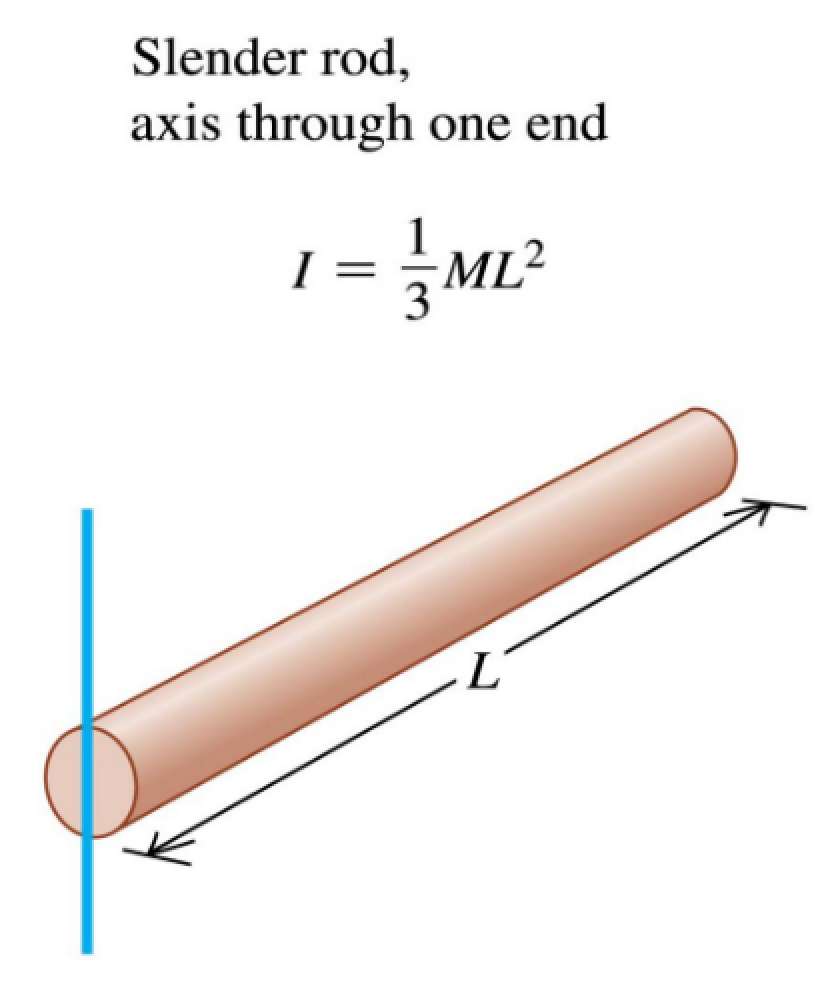
\includegraphics[width = 0.5\linewidth]{slender-rod-moi-2}
  \end{tabular}


  \section{Angular momentum}

  Angular momentum: \\
  \(\vec{L} = \vec{r} \times \vec{p}, \quad L = rp \sin \theta\) \\
  \(\vec{L} = \vec{r} \times m \vec{v}, \quad L = rmv \sin \theta\) \\
  \(\vec{L} = I \vec{\omega}, \quad L = I \omega\)

  Net torque: \\
  \(\vec{\tau}_{net} = \frac{dL}{dt}\) \\
  \(\vec{\tau}_{net} = I \vec{\alpha}, \quad \tau_{net} = I \alpha\)

  Angular velocity of precession: \\
  \(\Omega = \frac{\tau_{ext}}{L \sin \theta}\)


  \section{Electric Fields}

  Coulomb's law: \\
  \(F = \frac{1}{4 \pi \varepsilon_0} \frac{q_1 q_2}{r^2}\)

  Electric force: \\
  \(\vec{F} = q \vec{E}\)

  Electric field: \\
  \(\vec{E}_{net} = \int \frac{1}{4 \pi \varepsilon_0 r^2} \, dq\) \\
  \(\vec{E}_{net} = \sum_i \frac{q_i}{4 \pi \varepsilon_0 r^2}\)

  Electric field of a ring of charge: \\
  \(E = \frac{Q}{4 \pi \varepsilon_0} \frac{x}{(r^2 +x^2)^{\frac{3}{2}}}\)

  Electric field of a cylinder: \\
  \(E = \frac{1}{2 \pi \varepsilon_0} \frac{\lambda}{x}\)

  Electric field of a thin plane of charge: \\
  \(E = \frac{\sigma}{2 \varepsilon_0}\)

  Electric field at the surface of a conductor: \\
  \(E_{\perp} = \frac{\sigma}{\varepsilon_0}\)

  Electric field between two uniformly charged plates: \\
  \(E = \frac{V}{d}\)

  Dipole moment (\(-\) to \(+\)): \\
  \(p = qd\)

  Electric dipole torque: \\
  \(\vec{\tau} = \vec{p} \times \vec{E}, \quad \tau = pE \sin \theta = qd E \sin \theta\)

  Electric potential: \\
  \(V = \frac{U}{q}\) \\
  \(V = \frac{1}{4 \pi \varepsilon_0} \sum_i \frac{q_i}{r}\) \\
  \(V = - \int \vec{E} \, d \vec{r}\)

  Electric potential energy of 2 point charges: \\
  \(U = \frac{q_1 q_2}{4 \pi \varepsilon_0 r}\)

  Electric potential energy of a system of discrete charges: \\
  \(U = \frac{1}{2} \sum_i \sum_{j \ne i} \frac{q_i q_j}{4 \pi \varepsilon_0 r_{ij}}\)

  Electric potential energy of a dipole: \\
  \(U = - \vec{p} \cdot \vec{E} = - pE \cos \theta\)

  Electric flux: \\
  \(\Phi_E = \int \vec{E} \cdot d \vec{A} = E \cos \theta \, dA = EA \cos \theta\)

  Gauss' Law: \\
  \(\oint \vec{E} \cdot d \vec{A} = \frac{Q_{encl}}{\varepsilon_0}\)


  \section{DC Circuits}

  Resistance: \\
  \(R = \frac{V}{I}\)

  Resistors in series: \\
  \(R_{eq} = R_1 + R_2 + \cdots\)

  Resistors in parallel: \\
  \(R_{eq} = \left(\frac{1}{R_1} + \frac{1}{R_2} + \cdots \right)^{-1}\)

  Electromotive force (e.m.f): \\
  \(\mathcal{E} = \frac{W}{Q}\)

  Internal resistance \(r\): \\
  \(V_{\text{terminal}} = \mathcal{E} - Ir\)

  Power (replace \(R\) with \(X_C\) or \(X_L\) for AC): \\
  \(P = VI = I^2 R = \frac{V^2}{R}\)

  Potential divider: (replace \(R\) with \(R, X_C\) or \(X_L\) and \(R_{total}\) with \(Z\) for AC) \\
  \(V = \frac{R}{R_{total}} V_{total}\)

  Capacitance: \\
  \(C = \frac{Q}{V} = \frac{\varepsilon_0 A}{d}\)

  Capacitance of a conducting sphere: \\
  \(C = 4 \pi \varepsilon_0 r\)

  Capacitance of a co-axial cylindrical conductor: \\
  \(C = \frac{2 \pi \varepsilon_0 L}{\ln \left| \frac{R_{out}}{R_{in}} \right|}\)

  Capacitors in series: \\
  \(C_{eq} = \left(\frac{1}{C_1} + \frac{1}{C_2} + \cdots \right)^{-1}\)

  Capacitors in parallel: \\
  \(C_{eq} = C_1 + C_2 + \cdots\)

  Potential energy stored in a capacitor: \\
  \(U = \frac{1}{2} \frac{Q^2}{C} = \frac{1}{2} CV^2 = \frac{1}{2} QV\)

  Electric energy density in a vacuum: \\
  \(u = \frac{1}{2} \varepsilon_0 E^2\)

  Electric energy density in the presence of a dielectric: \\
  \(u = \frac{1}{2} \varepsilon_r \varepsilon_0 E^2 = \frac{1}{2} K \varepsilon_0 E^2 = \frac{1}{2} \varepsilon E^2\)

  Capacitance with a dielectric: \\
  \(C = KC_0 = K \frac{\varepsilon_0 A}{d} = \varepsilon \frac{A}{d}\)

  Gauss' Law in dielectrics: \\
  \(\oint K \vec{E} \cdot d \vec{A} = \frac{Q_{encl-free}}{\varepsilon_0}\)

  Charging a capacitor: \\
  \(q = C \mathcal{E} \left( 1 - e^{- \frac{t}{RC}} \right) = Q_f \left(1 - e^{- \frac{t}{RC}} \right)\) \\
  \(i = \frac{dq}{dt} = \frac{\mathcal{E}}{R} e^{-\frac{t}{RC}} = I_0 e^{-\frac{t}{RC}}\)

  Discharging a capacitor: \\
  \(q = Q_0 e^{- \frac{t}{RC}}\) \\
  \(i = -\frac{dq}{dt} = -\frac{Q_0}{RC} e^{-\frac{t}{RC}} = I_0 e^{-\frac{t}{RC}}\)

  Applying Kirchhoff's laws: \\
  \(- \rightarrow +\) (Increasing \(V\)) \(\longrightarrow\) Add \(V\) \\
  \(+ \rightarrow -\) (Decreasing \(V\)) \(\longrightarrow\) Subtract \(V\)

  \subsection{Capacitors in circuits}
  \(\lozenge\) When a capacitor is uncharged, it acts like a wire. \\
  \(\lozenge\) When a capacitor is fully charged, it acts like a break in the circuit. \\
  \(\lozenge\) When two charged capacitors are connected, the charges will transfer until the potential difference is the same for both capacitors. \\
  \(\lozenge\) When the capacitors' \textbf{same} polarity plates are connected together, the total charge is \(Q_1 + Q_2\), so the potential difference is \(\frac{Q_1 + Q_2}{C_1 + C_2}\) \\
  \(\lozenge\) When the capacitors' \textbf{opposite} polarity plates are connected together, the total charge is \(Q_1 - Q_2\), so the potential difference is \(\frac{Q_1 - Q_2}{C_1 + C_2}\) \\


  \section{Magnetic fields}

  Biot-Savart law for moving point charge: \\
  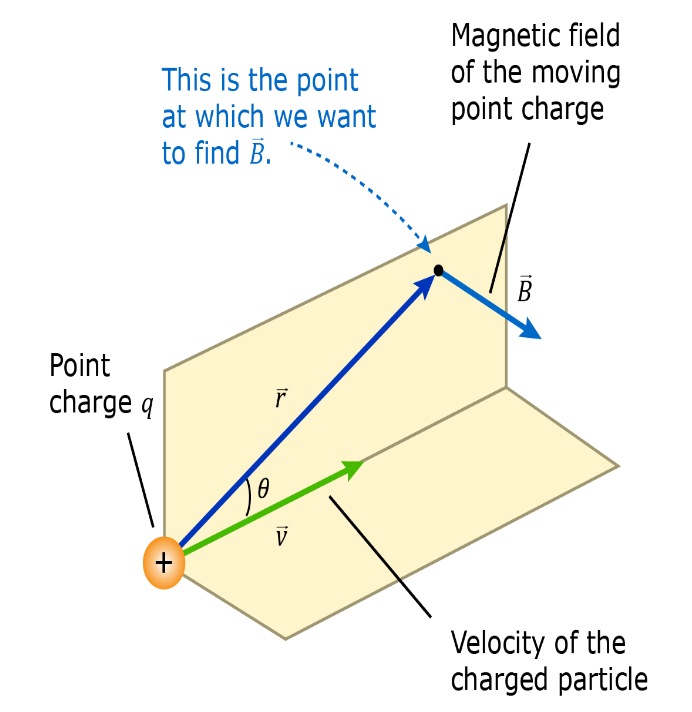
\includegraphics[width = 0.7\linewidth]{biot-savart-law-moving-charge}
  \(\vec{B} = \frac{\mu_0}{4 \pi} \frac{q \vec{v} \times \hat{r}}{r^2}\)

  Biot-Savart law for a current: \\
  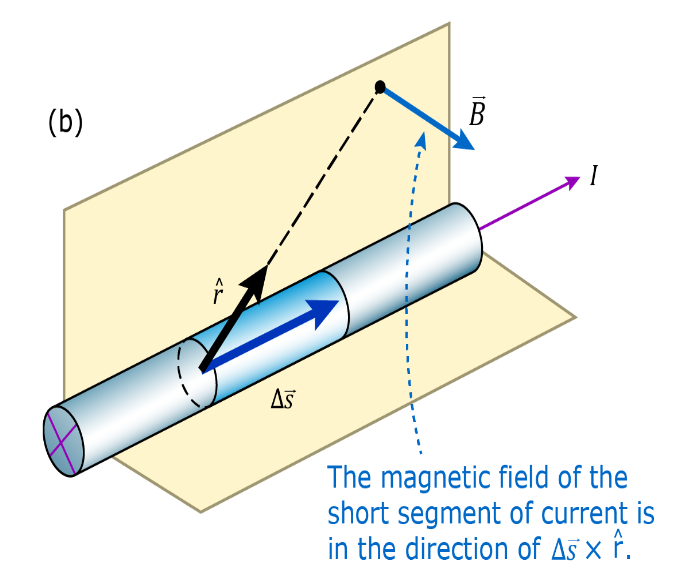
\includegraphics[width = 0.7\linewidth]{biot-savart-law-wire} \\
  \(d \vec{B} = \frac{\mu_0}{4 \pi} \frac{I \, d \vec{s} \times \hat{r}}{r^2}\)

  Ampere's law: \\
  \(\oint \vec{B} \cdot d \vec{l} = \mu_0 I_{encl}\) \\
  Use the right-hand grip rule to determine the direction of the current \(I_{encl}\).

  Magnetic flux: \\
  \(\Phi_B = \int \vec{B} \cdot d \vec{A} = \int B \cos \phi \, dA = BA \cos \phi\)

  Gauss' law: \\
  \(\oint \vec{B} \cdot d \vec{A} = 0\)

  Force on a moving charge in a magnetic field: \\
  \(\vec{F} = q \vec{v} \times \vec{B}, \quad F = Bqv \sin \theta\)

  Lorentz force: \\
  \(\vec{F} = q \vec{E} + q \vec{v} \times \vec{B}\)

  Force on a current in a magnetic field: \\
  \(\vec{F} = I \vec{l} \times \vec{B}\) \\
  \(F = BIl \sin \theta\)

  Magnetic field of a solenoid: \\
  \(B = \mu_0 n I\)

  Magnetic dipole moment: \\
  \(\vec{\mu} = NI \vec{A}\)

  Magnetic dipole torque: \\
  \(\vec{\tau} = \vec{\mu} \times \vec{B}\) \\
  \(\tau = \mu B \sin \theta = NIAB \sin \theta\)

  Velocity selector: \\
  \(v = \frac{E}{B_{in}}\)

  Mass spectrometer: \\
  \(m = \frac{B_{in}B_1 Rq}{E}\)

  Hall voltage: \\
  \(\Delta V_H = E_H d = v_d B d\)


  \section{Electromagnetic induction}

  Magnetic flux linkage: \\
  \(N \Phi_B = N \int \vec{B} \cdot d \vec{A} = NBA \cos \theta\)

  Faraday's law: \\
  \(\mathcal{E} = -N \frac{d \Phi_B}{dt}\)

  E.m.f induced in a moving conductor: \\
  \(\mathcal{E} = Blv \sin \theta\)

  Maxwell-Faraday law: \\
  \(\mathcal{E} = \oint \vec{E} \cdot d \vec{l} = - \frac{d \Phi_B} {dt}\) \\
  \(\oint \vec{E} \cdot d \vec{l} \ne 0\)

  Ampere-Maxwell law: \\
  \(\oint \vec{B} \cdot d \vec{l} = \mu_0 \left( I_{encl} + I_{disp} \right)\) \\
  \(\oint \vec{B} \cdot d \vec{l} = \mu_0 \left( I_{encl} + \varepsilon_0 \frac{d \Phi_E}{dt} \right)\) \\
  \(\oint \vec{B} \cdot d \vec{l} = \mu_0 \left( I_{encl} + \varepsilon_0 A \frac{dE}{dt} \right)\)

  Mutual inductance: \\
  \(M = \frac{N_2 \Phi_{B2}}{I_1} = \frac{N_1 \Phi_{B1}}{I_2}\)

  Self inductance: \\
  \(L = \frac{N \Phi_B}{I}\)

  Energy stored in the magnetic field: \\
  \(U_B = \frac{1}{2} LI^2\)

  AC generators: \\
  \(\mathcal{E} = NBA \omega \sin \omega t\)

  Transformer: \\
  \(\frac{V_s}{V_p} = \frac{N_s}{N_p}\) \\
  \(V_p I_p = V_s I_s\)


  \section{Inductors}

  Potential difference across an inductor: \\
  \(V = L \frac{dI}{dt}\)

  Inductors in series: \\
  \(L_{eq} = L_1 + L_2 + \cdots\)

  Inductive reactance: \\
  \(X_L = \omega L = 2 \pi f L\)

  Capacitive reactance: \\
  \(X_C = \frac{1}{\omega C} = \frac{1}{2 \pi fC}\)

  Resonance in AC circuits: \\
  Condition for resonance is: \(X_C = X_L\) \\
  \(f_0 = \frac{\omega_0}{2 \pi} = \frac{1}{2 \pi} \sqrt{\frac{1}{LC}}\)

  \subsection{RL series circuit}

  Current: \\
  \(I = \frac{V_0}{R} \left(1 - e^{-\frac{Rt}{L}} \right)\)

  \subsection{LC circuit (no voltage source)}

  Charge: \\
  \(Q = Q_0 \cos \left( \omega t + \phi \right)\)

  Angular frequency: \\
  \(\omega = 2 \pi f = \sqrt{\frac{1}{LC}}\)

  Total energy: \\
  \(U = \frac{Q_0^2}{2C}\)

  \subsection{RCL series circuit (no V source)}

  Angular frequency (under-damped oscillations): \\
  \(\omega' = \sqrt{\frac{1}{LC} - \frac{R^2}{4L^2}}\)

  Charge: \\
  \(Q = Q_0 e^{-\frac{Rt}{2L}} \cos (\omega ' t + \phi)\)

  \subsection{RCL series circuit}

  \textbf{Phasor diagram} \\
  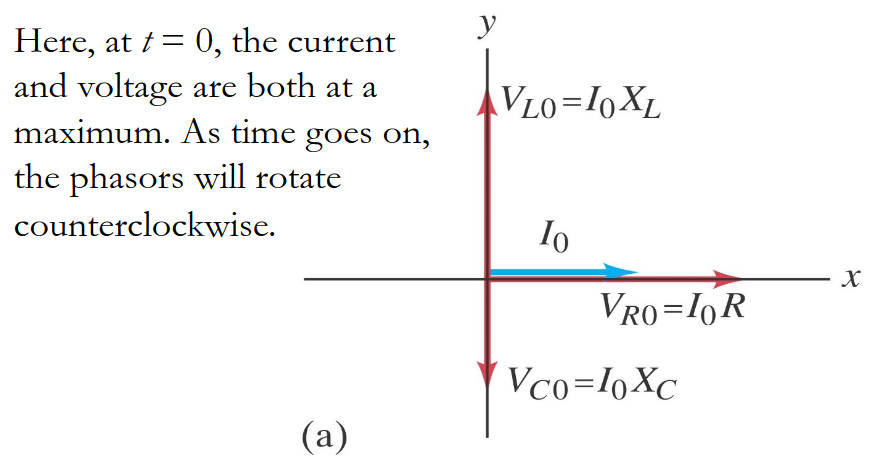
\includegraphics[width = 0.95\linewidth]{rcl-circuit-phasor-diagram-1}
  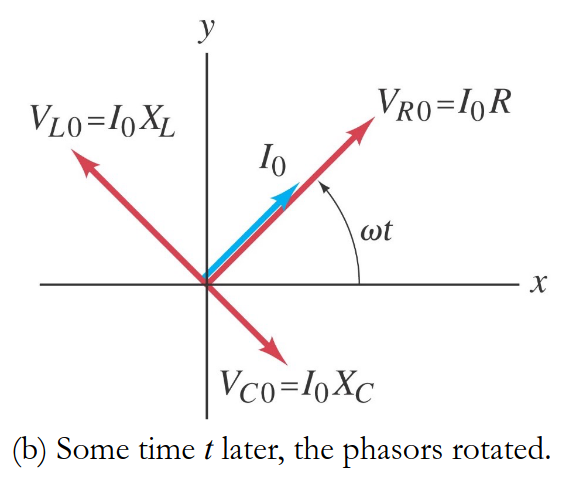
\includegraphics[width = 0.95\linewidth]{rcl-circuit-phasor-diagram-2}
  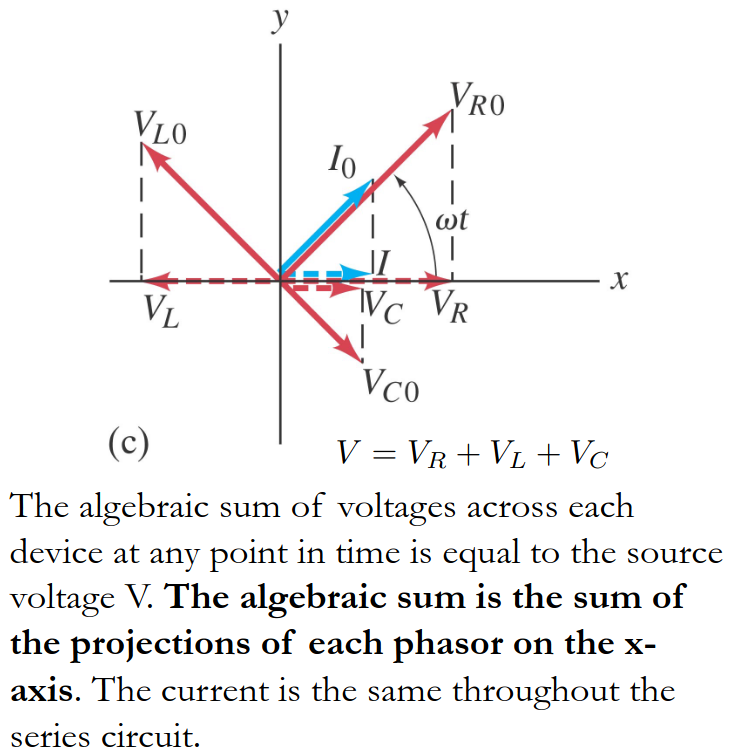
\includegraphics[width = \linewidth]{rcl-circuit-phasor-diagram-3}

  Impedance: \\
  \(Z = \sqrt{R^2 + \left(\omega L - \frac{1}{\omega C} \right)^2}\)

  Current: \\
  \(I = I_0 \cos \omega t\)

  Voltage: \\
  \(V = I_0 Z \cos (\omega t + \phi)\)

  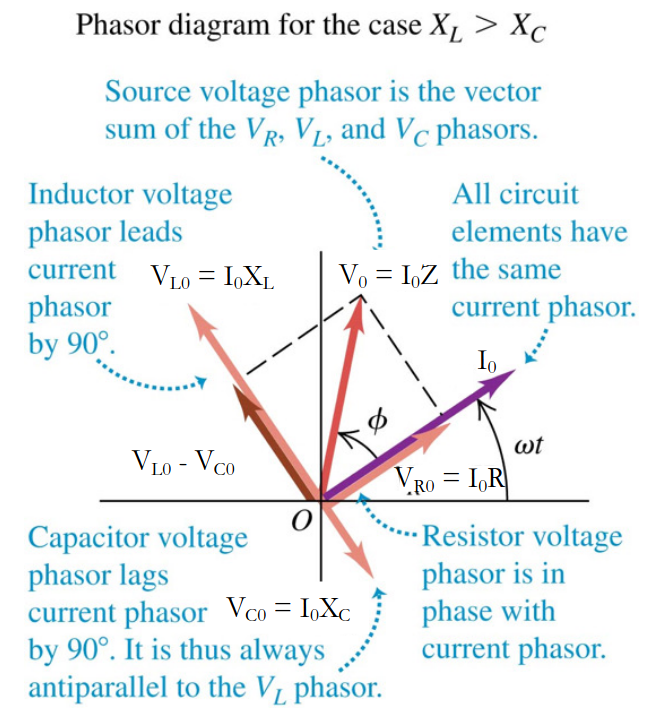
\includegraphics[width = \linewidth]{rcl-circuit-phasor-diagram-phase-angle}

  Phase angle between voltage and current: \\
  \(\phi = \arctan \left(\frac{X_L - X_C}{R} \right)\)

  \subsection{Resistors in AC circuits}

  Root-mean-square current: \\
  \(I_{rms} = \frac{I_0}{\sqrt{2}}\) \\
  The current through a resistor is \textbf{in phase} with the voltage.

  \subsection{Inductors in AC circuits}

  Voltage: \\
  \(V = \omega L I_0 \cos \left( \omega t + \frac{\pi}{2} \right) = V_0 \cos \left(\omega t + \frac{\pi}{2} \right)\)

  Current: \\
  \(I_0 = \frac{V_0}{\omega L}\) \\
  The current through an inductor \textbf{lags} the voltage by \(90^{\circ}\).

  \subsection{Capacitors in AC circuits}

  Voltage: \\
  \(V = \frac{I_0}{\omega C} \cos \left( \omega t - \frac{\pi}{2} \right) = V_0 \cos \left( \omega t - \frac{\pi}{2} \right)\)

  Current: \\
  \(I_0 = V_0 \omega C\) \\
  The current through a capacitor \textbf{leads} the voltage by \(90^{\circ}\).

  \subsection{Filter circuits}
  Use potential divider equation (under DC circuits) for all filter circuits.

  \section{Trigonometric identities}

  % Quotient identities: \\
  % \(\tan \theta = \frac{\sin \theta}{\cos \theta}\) \\
  % \(\cot \theta = \frac{\cos \theta}{\sin \theta}\)

  % Reciprocal identities: \\
  % \(\sin \theta = \frac{1}{\csc \theta}\) \\
  % \(\csc \theta = \frac{1}{\sin \theta}\) \\
  % \(\cos \theta = \frac{1}{\sec \theta}\) \\
  % \(\sec \theta = \frac{1}{\cos \theta}\) \\
  % \(\tan \theta = \frac{1}{\cot \theta}\) \\
  % \(\cot \theta = \frac{1}{\tan \theta}\)

  Pythagorean identities: \\
  \(\sin^2 \theta + \cos^2 \theta = 1\) \\
  \(\sec^2 \theta - \tan^2 \theta = 1\) \\
  \(\csc^2 \theta - \cot^2 \theta = 1\)

  % Even/odd identities: \\
  % \(\sin(- \theta) = - \sin \theta\) \\
  % \(\cos (- \theta) = \cos \theta\) \\
  % \(\tan(- \theta) = - \tan \theta\) \\
  % \(\cot (- \theta) = - \cot \theta\) \\
  % \(\csc(- \theta) = - \csc \theta\) \\
  % \(\sec (- \theta) = \sec \theta\)

  % Co-function identities: \\
  % \(\sin \left(\frac{\pi}{2} - \theta \right) = \cos \theta\) \\
  % \(\cos \left(\frac{\pi}{2} - \theta\right) = \sin \theta \) \\
  % \(\tan \left(\frac{\pi}{2} - \theta \right) = \cot \theta\) \\
  % \(\cot \left(\frac{\pi}{2} - \theta\right) = \tan \theta \) \\
  % \(\csc \left(\frac{\pi}{2} - \theta \right) = \sec \theta\) \\
  % \(\sec \left(\frac{\pi}{2} - \theta\right) = \csc \theta \) \\
  % \(\frac{\pi}{2} \text{ radians} = 90^{\circ}\)

  % Sum/difference identities: \\
  % \(\sin (\theta \pm \phi) = \sin \theta \cos \phi \pm \cos \theta \sin \phi\) \\
  % \(\cos (\theta \pm \phi) = \cos \theta \cos \phi \mp \sin \theta \sin \phi\) \\
  % \(\tan (\theta \pm \phi) = \frac{\tan \theta \pm \tan \phi}{1 \mp \tan \theta \tan \phi}\) \\

  Double angle identities: \\
  \(\sin (2 \theta) = 2 \sin \theta \cos \theta\) \\
  \(\cos (2 \theta) = \cos^2 \theta - \sin^2 \theta\) \\
  \(\cos (2 \theta) = 2 \cos^2 \theta - 1\) \\
  \(\cos (2 \theta) = 1 - 2 \sin^2 \theta\) \\
  \(\tan (2 \theta) = \frac{2 \tan \theta}{1 - \tan^2 \theta}\)

  % Half angle identities: \\
  % \(\sin^2 \theta = \frac{1 - \cos (2 \theta)}{2}\) \\
  % \(\cos^2 \theta = \frac{1 + \cos (2 \theta)}{2}\) \\
  % \(\tan^2 \theta = \frac{1 - \cos (2 \theta)}{1 + \cos (2 \theta)}\)

  % Sum to product of 2 angles: \\
  % \(\sin \theta + \sin \phi = 2 \sin \left( \frac{\theta + \phi}{2} \right) \cos \left( \frac{\theta - \phi}{2} \right)\) \\
  % \(\sin \theta - \sin \phi = 2 \cos \left( \frac{\theta + \phi}{2} \right) \sin \left( \frac{\theta - \phi}{2} \right)\) \\
  % \(\cos \theta + \cos \phi = 2 \cos \left( \frac{\theta + \phi}{2} \right) \cos \left( \frac{\theta - \phi}{2} \right)\) \\
  % \(\cos \theta - \cos \phi = - 2 \sin \left( \frac{\theta + \phi}{2} \right) \sin \left( \frac{\theta - \phi}{2} \right)\)

  % Product to sum of 2 angles: \\
  % \(\sin \theta \sin \phi = \frac{\cos (\theta - \phi) - \cos (\theta + \phi)}{2}\) \\
  % \(\cos \theta \cos \phi = \frac{\cos (\theta - \phi) + \cos (\theta + \phi)}{2}\) \\
  % \(\sin \theta \cos \phi = \frac{\sin (\theta + \phi) + \sin (\theta - \phi)}{2}\) \\
  % \(\cos \theta \sin \phi = \frac{\sin (\theta + \phi) - \sin (\theta - \phi)}{2}\)

  Law of sines: \\
  \(\frac{a}{\sin A} = \frac{b}{\sin B} = \frac{c}{\sin C}\)

  Law of cosines: \\
  \(a^2 = b^2 + c^2 - 2bc \cos A\)

  Area of a triangle: \\
  \(A = \frac{1}{2} ab \sin C\)


  \section{Coordinates}
  Polar coordinates: \\
  \(x = r \cos \theta, \quad y = r \sin \theta\)

  Cylindrical coordinates: \\
  \(x = r \cos \theta, \quad y = r \sin \theta, \quad z = z\)

  Spherical coordinates: \\
  \(x = r \sin \theta \cos \phi\) \\
  \(y = r \sin \theta \sin \phi\) \\
  \(z = r \cos \theta\)


  \section{Steps}

  \subsection{General steps}
  \(\lozenge\) Always quote formula first. \\
  \(\lozenge\) Draw diagrams. \\
  \(\lozenge\) Change the formula's quantity, \(dm, dq\), etc, into something \(\times\) the given quantity. \\
  \(\lozenge\) Use symmetry to cancel things out. \\
  \(\lozenge\) Integration too hard? Substitute polar, cylindrical or spherical coordinates. \\
  \(\lozenge\) Infinity as a limit? Substitute with a \(\tan \theta\) as \(\tan \left(\pm \frac{\pi}{2} \right) \rightarrow \pm \infty\).

  \subsection{Steps to find centre of mass}
  \(\lozenge\) For discrete masses, treat holes as a mass but subtract them. \\
  \(\lozenge\) For continuous masses, change \(dm\) into something \(\times\) the given quantity, like \(\rho \, dV, \rho h \, dA, 2 \pi r \rho h \, dr\) for a cylinder.

  \subsection{Steps to find moment of inertia}
  \(\lozenge\) Find a symmetrical axis of rotation. \\
  \(\lozenge\) For continuous masses, change \(dm\) into something \(\times\) the given quantity, like \(\rho \, dV, \rho h \, dA, 2 \pi r \rho h \, dr\) for a cylinder. \\
  \(\lozenge\) Use parallel or perpendicular axis theorem to find the MOI about the actual axis of rotation if necessary.

  \subsection{Steps to find E-field (continuous)}
  \(\lozenge\) Convert \(dq\) into the something \(\times\) the given quantity, like \(\lambda \, dx, \sigma \, dA, \rho \, dV\). \\
  \(\lozenge\) Note that \(x\) and \(r\) are different, \(r\) is the distance away from the charged object. \\
  \(\lozenge\) A lot of times, \(E_y\) will cancel out, so you only need to consider \(E_x\). \\
  \(\lozenge\) If the shape is difficult to integrate, identify a shape that you can stack to get the shape you want, like rings for a disk and disks for a sphere.

  \subsection{Using Gauss' law}
  \(\lozenge\) Try to use a symmetrical surface. \\
  \(\lozenge\) Split the surface into sections, like the ends and the curved portion of a cylinder should be considered separately.

  \subsection{Using Ampere's law}
  \(\lozenge\) Generally, you want to use either a circle or a rectangle for the loop. \\
  \(\lozenge\) A circle is the easiest, as the B-field at every point on the circle is the same. \\
  \(\lozenge\) Using a rectangle, you will have to add the B-field of every side of the rectangle together to get the overall B-field.

\end{multicols*}
\end{document}